\subsection{Pixel size, magnification and resolution}
Our result from calculating how many pixels in the image (see figure \ref{fig:TestChart}) that corresponds to one centimeter were 41. When we calculated the length of a car in the image (see figure \ref{fig:Toy1}) we got the result 10 cm. When comparing the resolution from two images (see figure \ref{fig:Toy1} and \ref{fig:Toy2}) of a object at different distances, we got the result of more pixels per cm when closer to the object.

\begin{figure}
	\centering
	\begin{subfigure}[b]{0.3\textwidth}
		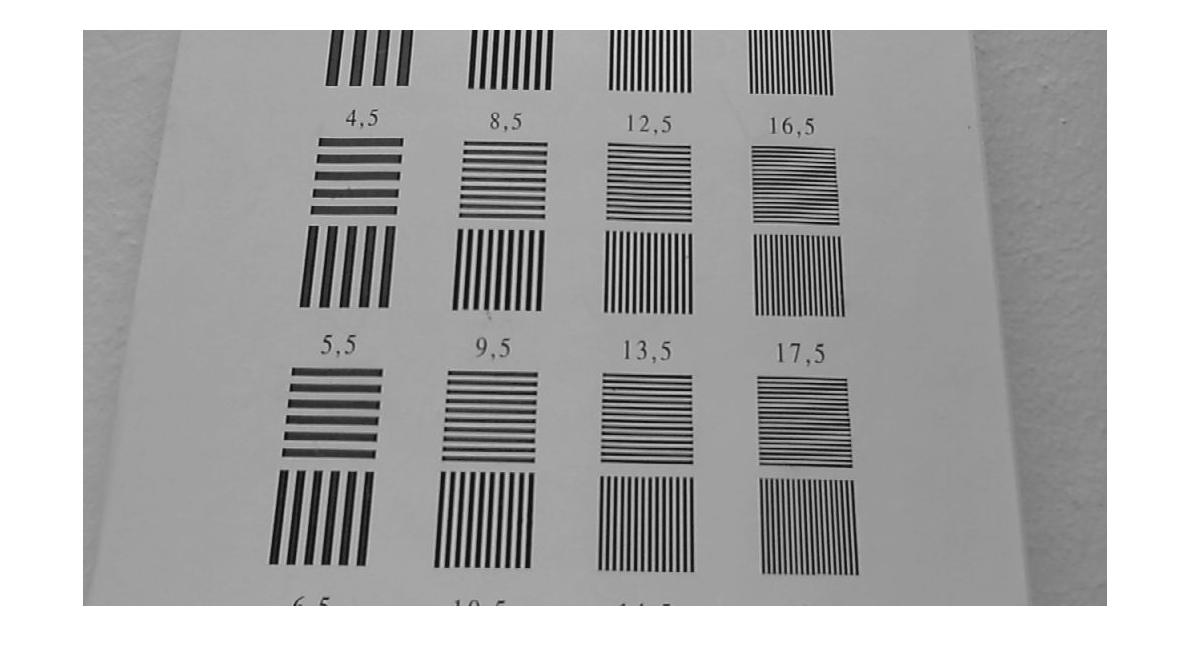
\includegraphics[width=\textwidth]{part1image1}
		\caption{}
		\label{fig:TestChart}
	\end{subfigure}
	\begin{subfigure}[b]{0.3\textwidth}
		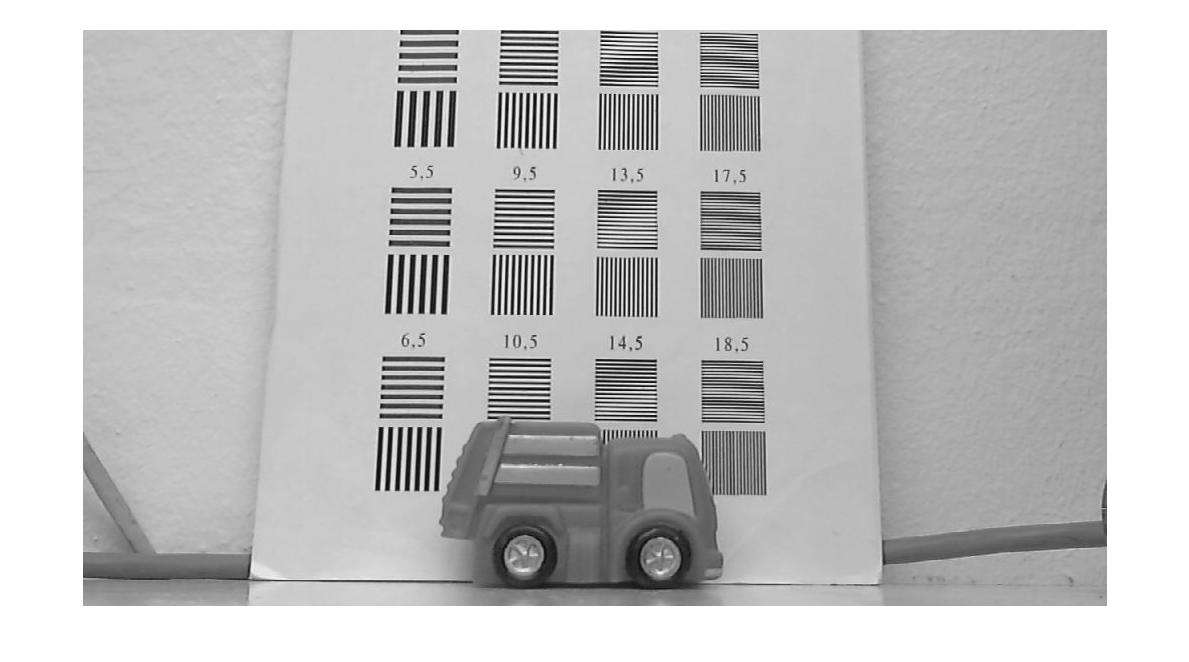
\includegraphics[width=\textwidth]{leksak1}
		\caption{}
		\label{fig:Toy1}
	\end{subfigure}
	\begin{subfigure}[b]{0.3\textwidth}
		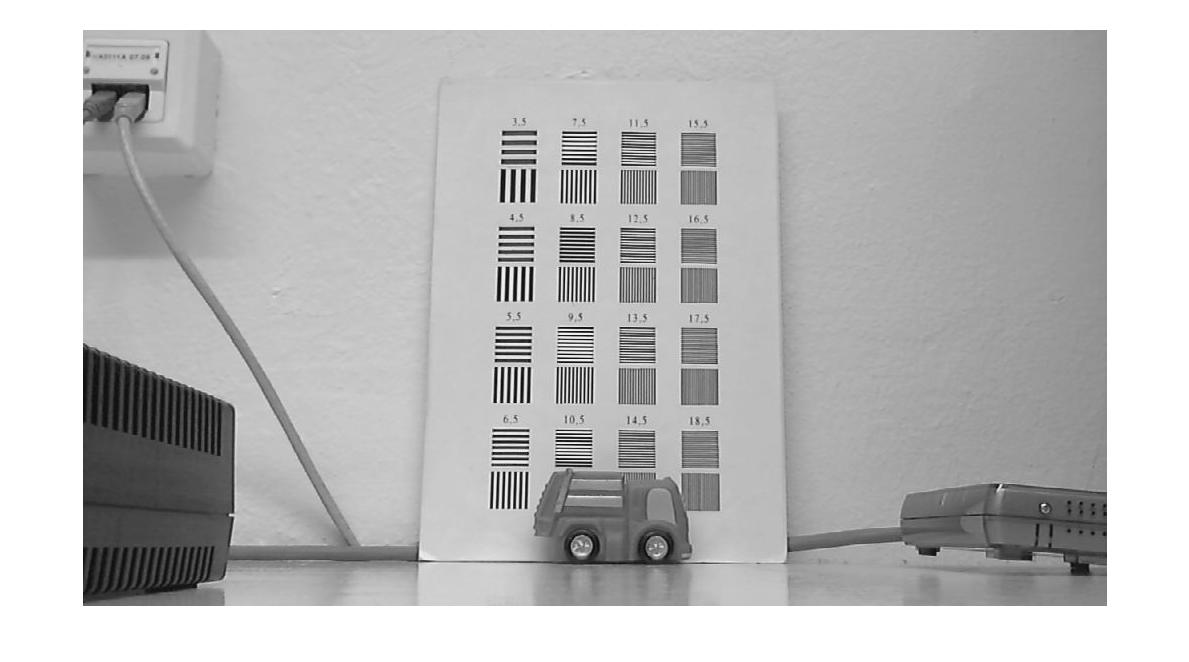
\includegraphics[width=\textwidth]{leksak2}
		\caption{}
		\label{fig:Toy2}
	\end{subfigure}
	\caption{(a) Image of test chart used to calculate how many pixels correspond to 1 cm. (b) Image used to measure distance of object and to compare the vertical and horizontal . (c) Image used to compare the resolution for different distances.}
	\label{fig:part1}
\end{figure}

\subsection{Grey scale images, image format and image information}
The result of using the function \texttt{mesh} can be seen in figure \ref{fig:meshCar}, and the result of using function \texttt{surfl} can be seen in figure \ref{fig:surflCar}), the functions \texttt{flipud} and \texttt{fliplr} flips the image vertically and horizontally respectively. 

The result of taking the matrix I2 and subtract with I1 we get an almost black image with the edges from the car (see figure \ref{fig:I2_I1})

The MTF-values for the image system in figure \ref{fig:Toy1} is shown in figure \ref{fig:mtf}

\begin{figure}
\centering
	\begin{subfigure}[b]{0.4\textwidth}
		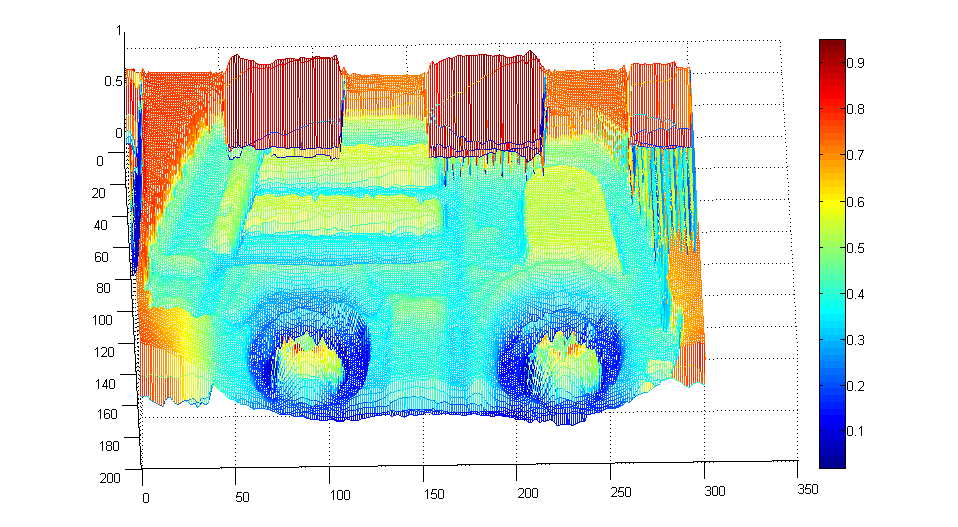
\includegraphics[width=\textwidth]{part2_mesh_croppedCar2}
		\caption{}
		\label{fig:meshCar}
	\end{subfigure}
	\begin{subfigure}[b]{0.4\textwidth}	
		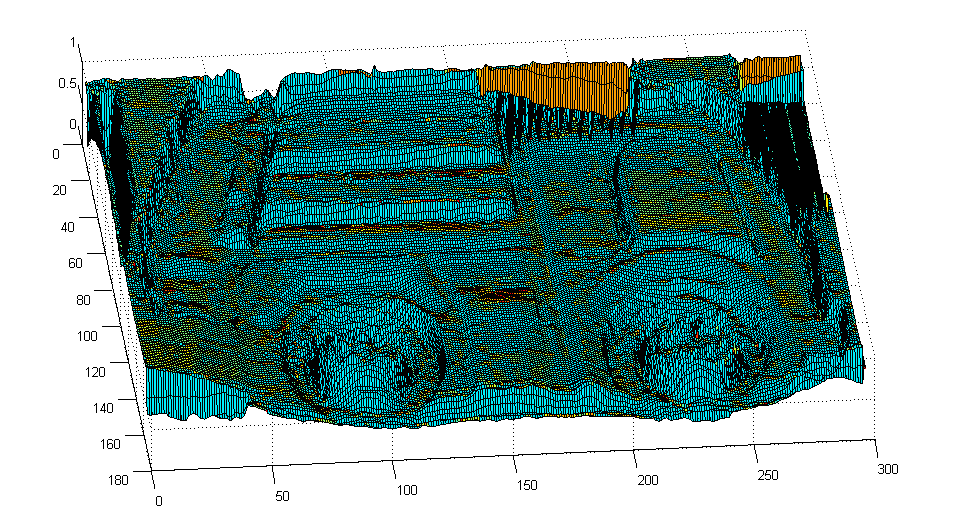
\includegraphics[width=\textwidth]{part2_surfl_croppedCar}
		\caption{}
		\label{fig:surflCar}
	\end{subfigure}
	\caption{(a) Matlab function \texttt{mesh} used on the cropped car image. (b) Matlab function \texttt{surfl} used on the cropped car image. }
	\label{fig:part2}
\end{figure}
\begin{figure}
	\centering
	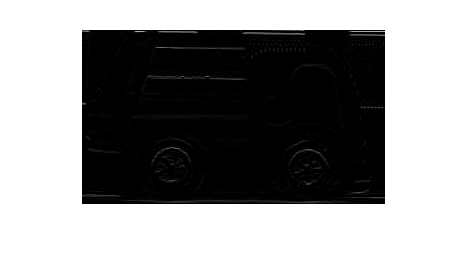
\includegraphics[width=0.5\textwidth]{part2_I1_I2}
	\caption{Subtracting a matrix with it self after shifted 1 pixel}
	\label{fig:I2_I1}
\end{figure}
\begin{figure}
	\centering
	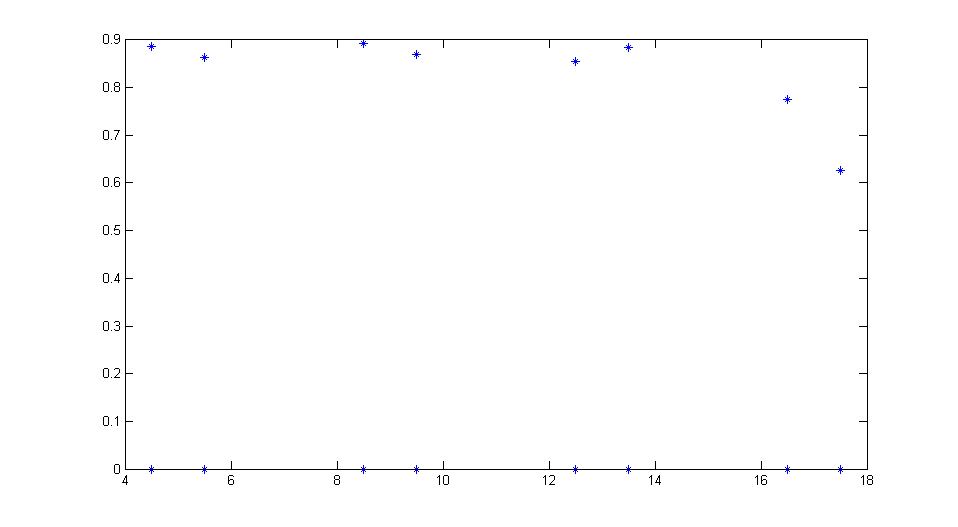
\includegraphics[width=0.5\textwidth]{part2_mtfdiagram}
	\caption{MTF-diagram for the image}
	\label{fig:mtf}
\end{figure}

\subsection{Image enhancement}
The results for image enhancement is seen in figure \ref{fig:img1new} and \ref{fig:img2new} the corresponding histogram is seen in figure \ref{fig:img1histnew} and \ref{fig:img2histnew}. The original images and there histograms can also be found in image \ref{fig:img1} and \ref{fig:img2}.
\begin{figure}
	\centering
	\begin{subfigure}[b]{0.4\textwidth}
		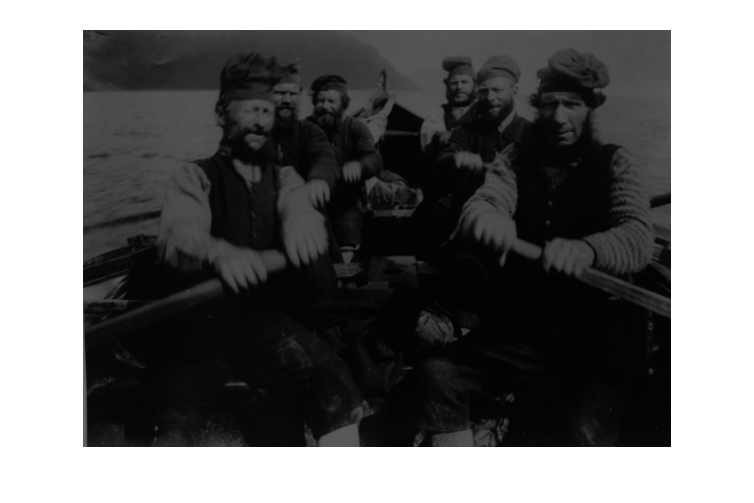
\includegraphics[width=\textwidth]{IE_img1org}
		\caption{}
		\label{fig:img1org}
	\end{subfigure}
	\begin{subfigure}[b]{0.4\textwidth}
		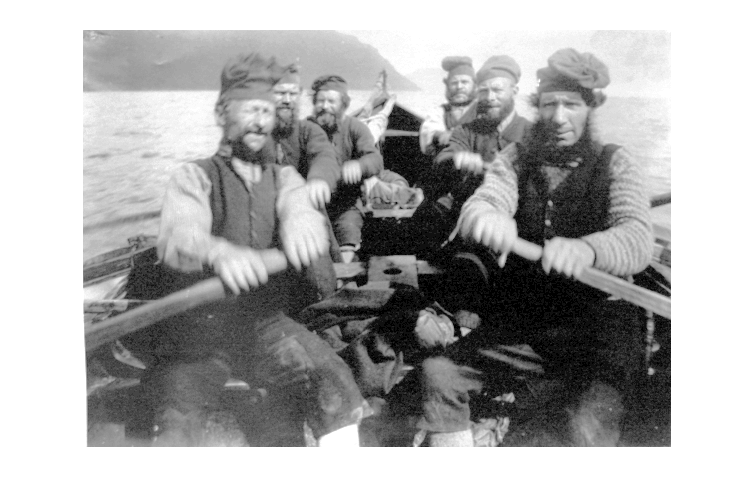
\includegraphics[width=\textwidth]{IE_img1New}
		\caption{}
		\label{fig:img1new}
	\end{subfigure}
	\\
	\begin{subfigure}[b]{0.4\textwidth}
		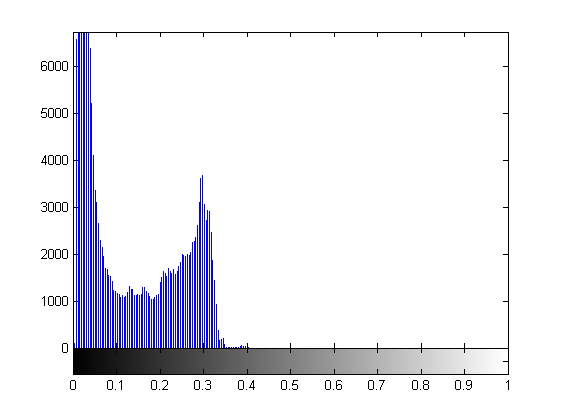
\includegraphics[width=\textwidth]{IE_img1_histOrg}
		\caption{}
		\label{fig:img1historg}
	\end{subfigure}
	\begin{subfigure}[b]{0.4\textwidth}
		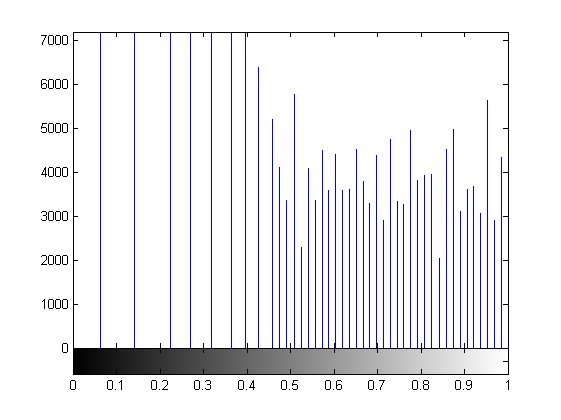
\includegraphics[width=\textwidth]{IE_img1_histNew}
		\caption{}
		\label{fig:img1histnew}
	\end{subfigure}
	\caption{(a) Original image. (b) Enhanced image. (c) Histogram for original image. (d) Histogram for enhanced image.}
	\label{fig:img1}
\end{figure}
\begin{figure}
	\centering
	\begin{subfigure}[b]{0.4\textwidth}
		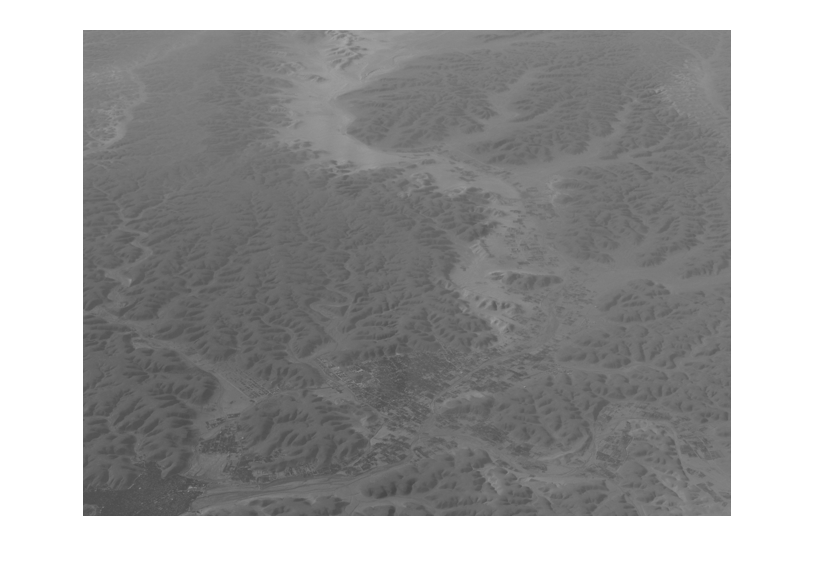
\includegraphics[width=\textwidth]{IE_img2org}
		\caption{}
		\label{fig:img2org}
	\end{subfigure}
	\begin{subfigure}[b]{0.4\textwidth}
		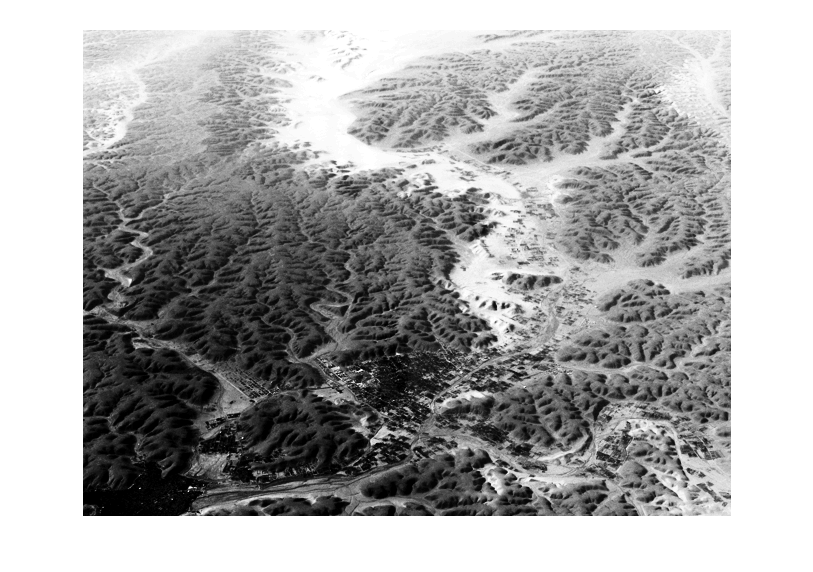
\includegraphics[width=\textwidth]{IE_img2New}
		\caption{}
		\label{fig:img2new}
	\end{subfigure}
	\\
	\begin{subfigure}[b]{0.4\textwidth}
		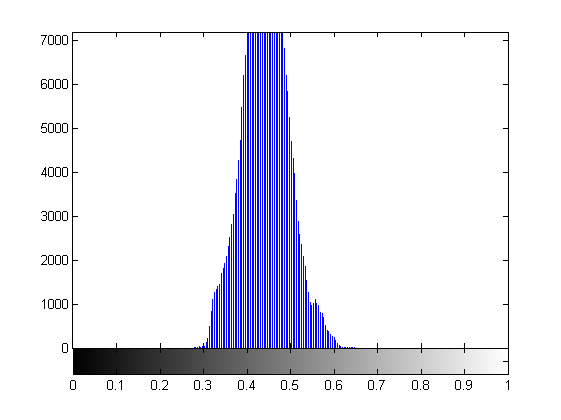
\includegraphics[width=\textwidth]{IE_img2_histOrg}
		\caption{}
		\label{fig:img2historg}
	\end{subfigure}
	\begin{subfigure}[b]{0.4\textwidth}
		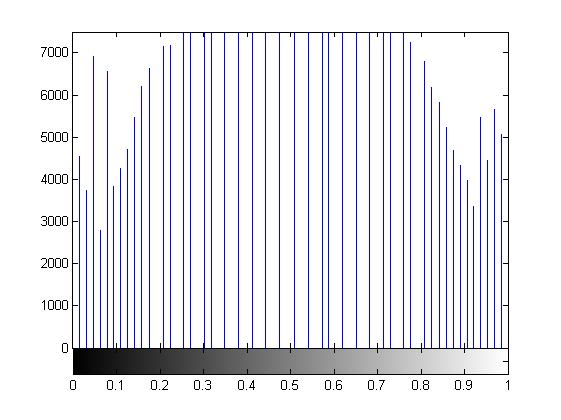
\includegraphics[width=\textwidth]{IE_img2_histNew}
		\caption{}
		\label{fig:img2histnew}
	\end{subfigure}
	\caption{(a) Original image. (b) Enhanced image. (c) Histogram for original image. (d) Histogram for enhanced image.}
	\label{fig:img2}
\end{figure}

\subsection{Colour images}
The results from using the function \texttt{anghist2} on a cropped red part (see figure \ref{fig:redCrop}) and a cropped blue part (see figure \ref{fig:blueCrop}) can be seen in figures \ref{fig:redSpec} and \ref{fig:blueSpec} respectively.

We plotted our observations from a cropped blue part of a car first by using a 3D plot RGB space (see figure \ref{fig:cartSpace}) and then by using sperical colour space (see figure \ref{fig:sphereSpace}).
\begin{figure}
	\centering
	\begin{subfigure}[b]{0.4\textwidth}
		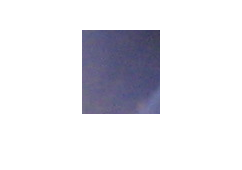
\includegraphics[width=\textwidth]{part4_bluecarcrop}
		\caption{A cropped blue part of a car}
		\label{fig:blueCrop}
	\end{subfigure}
	\begin{subfigure}[b]{0.4\textwidth}
		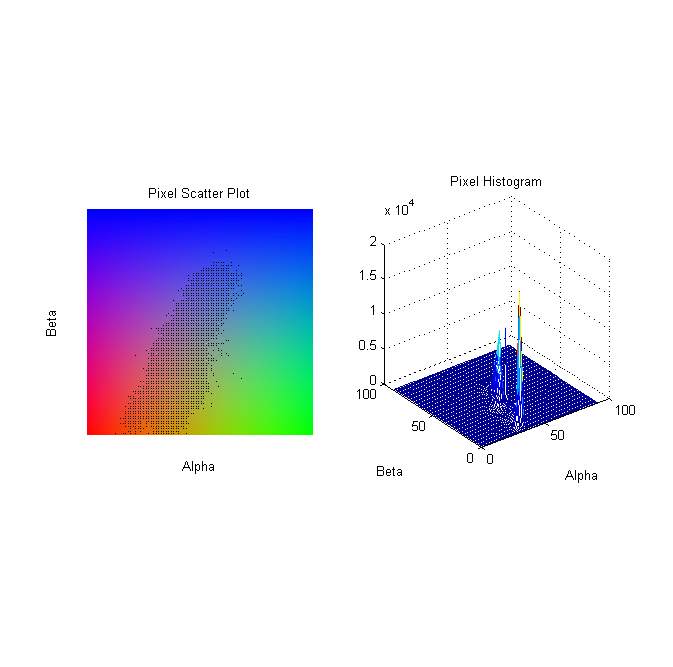
\includegraphics[width=\textwidth]{part4_anghist2_bluecar}
		\caption{Histogram on the blue part}
		\label{fig:blueSpec}
	\end{subfigure}
	\\
	\begin{subfigure}[b]{0.4\textwidth}
		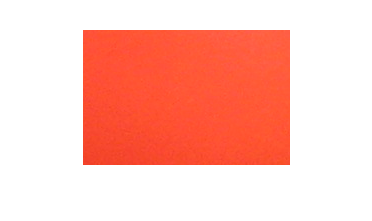
\includegraphics[width=\textwidth]{part4_smallredcrop}
		\caption{A cropped red part of a car}
		\label{fig:redCrop}
	\end{subfigure}
	\begin{subfigure}[b]{0.4\textwidth}
		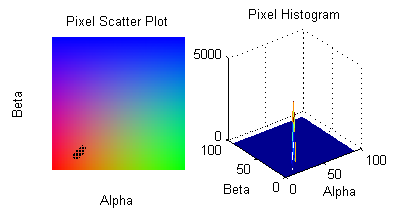
\includegraphics[width=\textwidth]{part4_anghist2_redcar}
		\caption{Histogram on the red part}
		\label{fig:redSpec}
	\end{subfigure}
	\caption{Histogram using function \texttt{anghist2}}
	\label{fig:colour}
\end{figure}
\begin{figure}

	\centering
	\begin{subfigure}[b]{0.4\textwidth}
		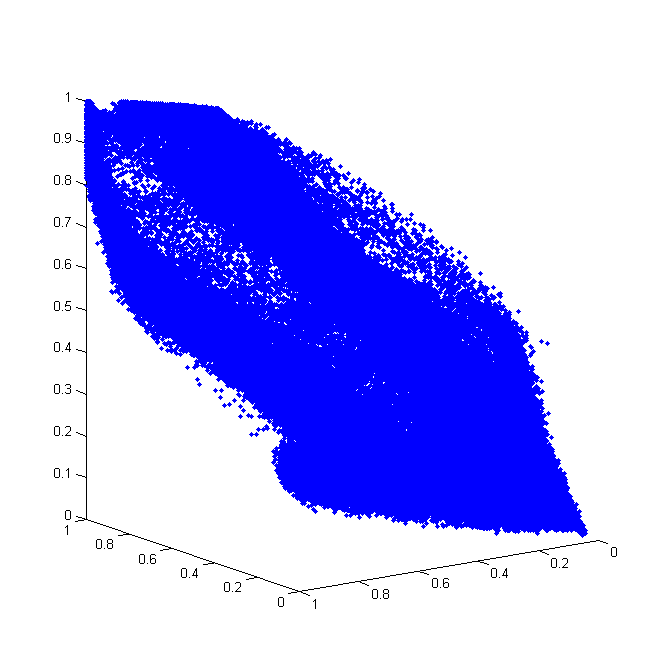
\includegraphics[width=\textwidth]{part4_cartspaceRGB_bluecar}
		\caption{}
		\label{fig:cartSpace}
	\end{subfigure}
	\begin{subfigure}[b]{0.4\textwidth}	
		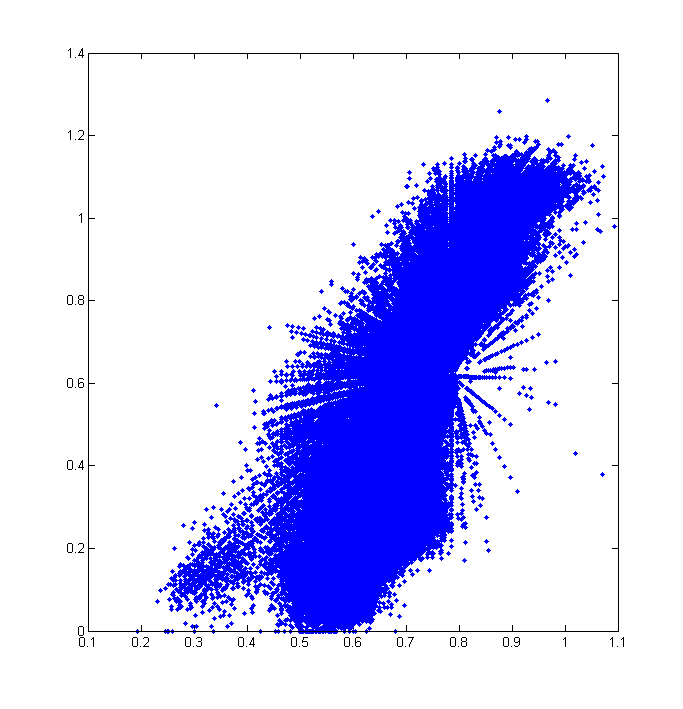
\includegraphics[width=\textwidth]{part4_spherespaceRGB_bluecar_plot}
		\caption{}
		\label{fig:sphereSpace}
	\end{subfigure}
	\caption{Two different ways to plot observations, (a) RGB space (b) spherical colour space. }
	\label{fig:part4Sphere}
\end{figure}

\subsection{IR - Imaging}
The visibility of a hand when using an IR camera depends on the object that blocks the hand from the camera and the results can be seen in figure \ref{fig:hand}. The reflections from a window and a whiteboard can be seen in figure \ref{fig:ref}. The result of heating up a plastic roller with two hands can be seen in figure \ref{fig:heat}.
\begin{figure}
	\centering
	\begin{subfigure}[b]{0.4\textwidth}
		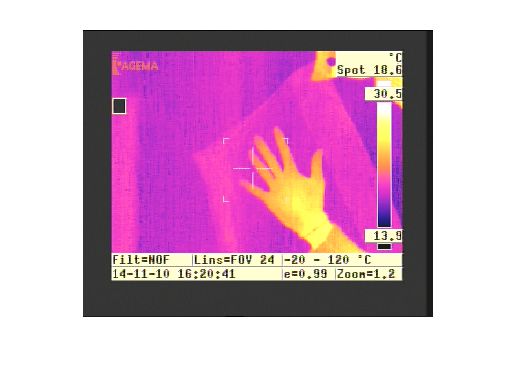
\includegraphics[width=\textwidth]{white_plasticbag}
		\caption{}
		\label{fig:whiteBag}
	\end{subfigure}
	\begin{subfigure}[b]{0.4\textwidth}
		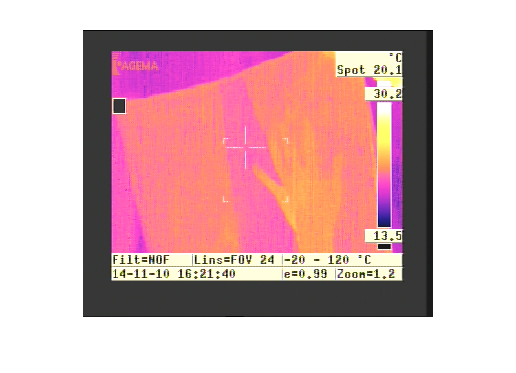
\includegraphics[width=\textwidth]{black_bag}
		\caption{}
		\label{fig:blackBag}
	\end{subfigure}
	\\
	\begin{subfigure}[b]{0.4\textwidth}
		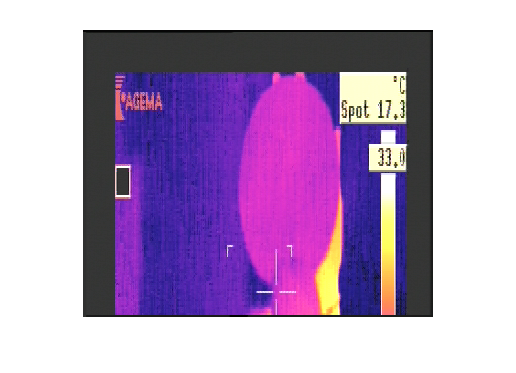
\includegraphics[width=\textwidth]{glass}
		\caption{}
		\label{fig:glass}
	\end{subfigure}
	\begin{subfigure}[b]{0.4\textwidth}
		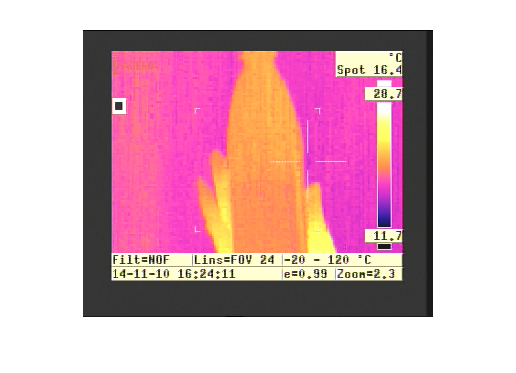
\includegraphics[width=\textwidth]{water_bottle}
		\caption{}
		\label{fig:waterBottle}
	\end{subfigure}
	\caption{Images taken with an IR camera of a hand behind different objects such as, (a) a white plastic bag, (b) a black plastic bag, (c) a circular object made out of glass and (d) a plastic bottle with water.}
	\label{fig:hand}
\end{figure}
\begin{figure}
	\centering
	\begin{subfigure}[b]{0.4\textwidth}
		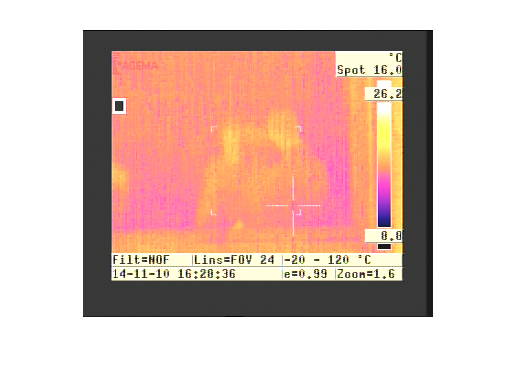
\includegraphics[width=\textwidth]{reflection}
		\caption{}
		\label{fig:refWin}
	\end{subfigure}
	\begin{subfigure}[b]{0.4\textwidth}
		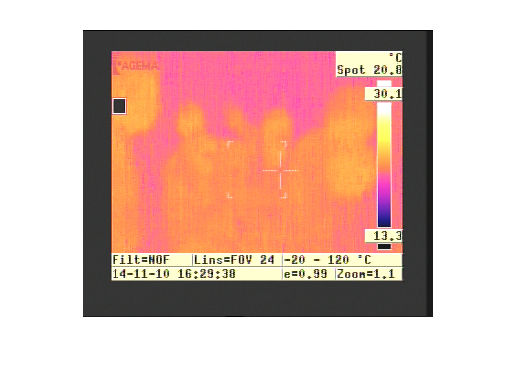
\includegraphics[width=\textwidth]{reflection_whiteboard}
		\caption{}
		\label{fig:refWB}
	\end{subfigure}
	\caption{Images taken with IR camera of reflections in (a) window and (b) whiteboard.}
	\label{fig:ref}
\end{figure}
\begin{figure}
	\centering
	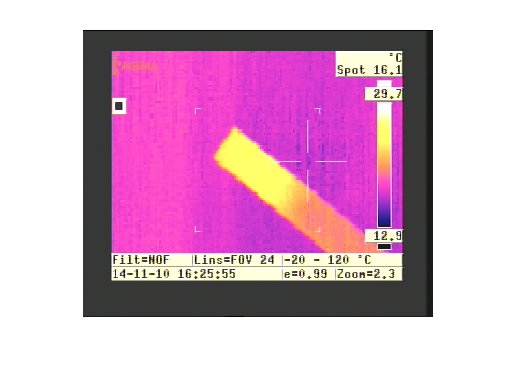
\includegraphics[width=0.5\textwidth]{heat}
	\caption{Image taken with IR camera of a heated plastic ruler.}
	\label{fig:heat}
\end{figure}